\documentclass[11pt,preprint, authoryear]{elsarticle}

\usepackage{lmodern}
%%%% My spacing
\usepackage{setspace}
\setstretch{1.2}
\DeclareMathSizes{12}{14}{10}{10}

% Wrap around which gives all figures included the [H] command, or places it "here". This can be tedious to code in Rmarkdown.
\usepackage{float}
\let\origfigure\figure
\let\endorigfigure\endfigure
\renewenvironment{figure}[1][2] {
    \expandafter\origfigure\expandafter[H]
} {
    \endorigfigure
}

\let\origtable\table
\let\endorigtable\endtable
\renewenvironment{table}[1][2] {
    \expandafter\origtable\expandafter[H]
} {
    \endorigtable
}


\usepackage{ifxetex,ifluatex}
\usepackage{fixltx2e} % provides \textsubscript
\ifnum 0\ifxetex 1\fi\ifluatex 1\fi=0 % if pdftex
  \usepackage[T1]{fontenc}
  \usepackage[utf8]{inputenc}
\else % if luatex or xelatex
  \ifxetex
    \usepackage{mathspec}
    \usepackage{xltxtra,xunicode}
  \else
    \usepackage{fontspec}
  \fi
  \defaultfontfeatures{Mapping=tex-text,Scale=MatchLowercase}
  \newcommand{\euro}{€}
\fi

\usepackage{amssymb, amsmath, amsthm, amsfonts}

\def\bibsection{\section*{References}} %%% Make "References" appear before bibliography


\usepackage[round]{natbib}

\usepackage{longtable}
\usepackage[margin=2.3cm,bottom=2cm,top=2.5cm, includefoot]{geometry}
\usepackage{fancyhdr}
\usepackage[bottom, hang, flushmargin]{footmisc}
\usepackage{graphicx}
\numberwithin{equation}{section}
\numberwithin{figure}{section}
\numberwithin{table}{section}
\setlength{\parindent}{0cm}
\setlength{\parskip}{1.3ex plus 0.5ex minus 0.3ex}
\usepackage{textcomp}
\renewcommand{\headrulewidth}{0.2pt}
\renewcommand{\footrulewidth}{0.3pt}

\usepackage{array}
\newcolumntype{x}[1]{>{\centering\arraybackslash\hspace{0pt}}p{#1}}

%%%%  Remove the "preprint submitted to" part. Don't worry about this either, it just looks better without it:
\makeatletter
\def\ps@pprintTitle{%
  \let\@oddhead\@empty
  \let\@evenhead\@empty
  \let\@oddfoot\@empty
  \let\@evenfoot\@oddfoot
}
\makeatother

 \def\tightlist{} % This allows for subbullets!

\usepackage{hyperref}
\hypersetup{breaklinks=true,
            bookmarks=true,
            colorlinks=true,
            citecolor=blue,
            urlcolor=blue,
            linkcolor=blue,
            pdfborder={0 0 0}}


% The following packages allow huxtable to work:
\usepackage{siunitx}
\usepackage{multirow}
\usepackage{hhline}
\usepackage{calc}
\usepackage{tabularx}
\usepackage{booktabs}
\usepackage{caption}


\newenvironment{columns}[1][]{}{}

\newenvironment{column}[1]{\begin{minipage}{#1}\ignorespaces}{%
\end{minipage}
\ifhmode\unskip\fi
\aftergroup\useignorespacesandallpars}

\def\useignorespacesandallpars#1\ignorespaces\fi{%
#1\fi\ignorespacesandallpars}

\makeatletter
\def\ignorespacesandallpars{%
  \@ifnextchar\par
    {\expandafter\ignorespacesandallpars\@gobble}%
    {}%
}
\makeatother

\newlength{\cslhangindent}
\setlength{\cslhangindent}{1.5em}
\newenvironment{CSLReferences}%
  {\setlength{\parindent}{0pt}%
  \everypar{\setlength{\hangindent}{\cslhangindent}}\ignorespaces}%
  {\par}


\urlstyle{same}  % don't use monospace font for urls
\setlength{\parindent}{0pt}
\setlength{\parskip}{6pt plus 2pt minus 1pt}
\setlength{\emergencystretch}{3em}  % prevent overfull lines
\setcounter{secnumdepth}{5}

%%% Use protect on footnotes to avoid problems with footnotes in titles
\let\rmarkdownfootnote\footnote%
\def\footnote{\protect\rmarkdownfootnote}
\IfFileExists{upquote.sty}{\usepackage{upquote}}{}

%%% Include extra packages specified by user

%%% Hard setting column skips for reports - this ensures greater consistency and control over the length settings in the document.
%% page layout
%% paragraphs
\setlength{\baselineskip}{12pt plus 0pt minus 0pt}
\setlength{\parskip}{12pt plus 0pt minus 0pt}
\setlength{\parindent}{0pt plus 0pt minus 0pt}
%% floats
\setlength{\floatsep}{12pt plus 0 pt minus 0pt}
\setlength{\textfloatsep}{20pt plus 0pt minus 0pt}
\setlength{\intextsep}{14pt plus 0pt minus 0pt}
\setlength{\dbltextfloatsep}{20pt plus 0pt minus 0pt}
\setlength{\dblfloatsep}{14pt plus 0pt minus 0pt}
%% maths
\setlength{\abovedisplayskip}{12pt plus 0pt minus 0pt}
\setlength{\belowdisplayskip}{12pt plus 0pt minus 0pt}
%% lists
\setlength{\topsep}{10pt plus 0pt minus 0pt}
\setlength{\partopsep}{3pt plus 0pt minus 0pt}
\setlength{\itemsep}{5pt plus 0pt minus 0pt}
\setlength{\labelsep}{8mm plus 0mm minus 0mm}
\setlength{\parsep}{\the\parskip}
\setlength{\listparindent}{\the\parindent}
%% verbatim
\setlength{\fboxsep}{5pt plus 0pt minus 0pt}



\begin{document}



%titlepage
\thispagestyle{empty}
\begin{center}
\begin{minipage}{0.75\linewidth}
    \centering
%Entry1
    {\uppercase{\huge Question 5 - Volatility and GARCH estimates\par}}
    \vspace{2cm}
%Author's name
    {\LARGE \textbf{Carel Olivier}\par}
    \vspace{1cm}
%University logo
\begin{center}
    
\includegraphics[width=\linewidth]{Tex/garch.png}
\end{center}
\vspace{1cm}
%Supervisor's Details
\begin{center}
    {\Large 22017542\par}
    \vspace{1cm}
%Degree
    {\large \par}
    \vspace{1cm}
%Institution
    {\large \par}
    \vspace{1cm}
%Date
    {\large }
%More
    {\normalsize }
%More
    {\normalsize }
\end{center}
\end{minipage}
\end{center}
\clearpage


\begin{frontmatter}  %

\title{}

% Set to FALSE if wanting to remove title (for submission)


\vspace{1cm}





\vspace{0.5cm}

\end{frontmatter}



%________________________
% Header and Footers
%%%%%%%%%%%%%%%%%%%%%%%%%%%%%%%%%
\pagestyle{fancy}
\chead{}
\rhead{}
\lfoot{}
\rfoot{\footnotesize Page \thepage}
\lhead{}
%\rfoot{\footnotesize Page \thepage } % "e.g. Page 2"
\cfoot{}

%\setlength\headheight{30pt}
%%%%%%%%%%%%%%%%%%%%%%%%%%%%%%%%%
%________________________

\headsep 35pt % So that header does not go over title




\hypertarget{short-introduction}{%
\section{Short Introduction}\label{short-introduction}}

The study of volatility is particularly important in financial
modelling. Thus, in this question I will look at the South African ZAR
since it has been quite volatile over the past couple of years. More
specifically, I will conduct a simple univariate-GARCH estimation to
analyse the volatility of the Rand.

\hypertarget{implied-volatility}{%
\section{Implied Volatility}\label{implied-volatility}}

I will start by looking at implied volatility. The market's estimate of
how much a currency pair will fluctuate over a certain period in the
future is known as implied volatility. Option traders can use a currency
volatility index to price options on currency pairs. Implied volatility
is generally considered a measure of sentiment.

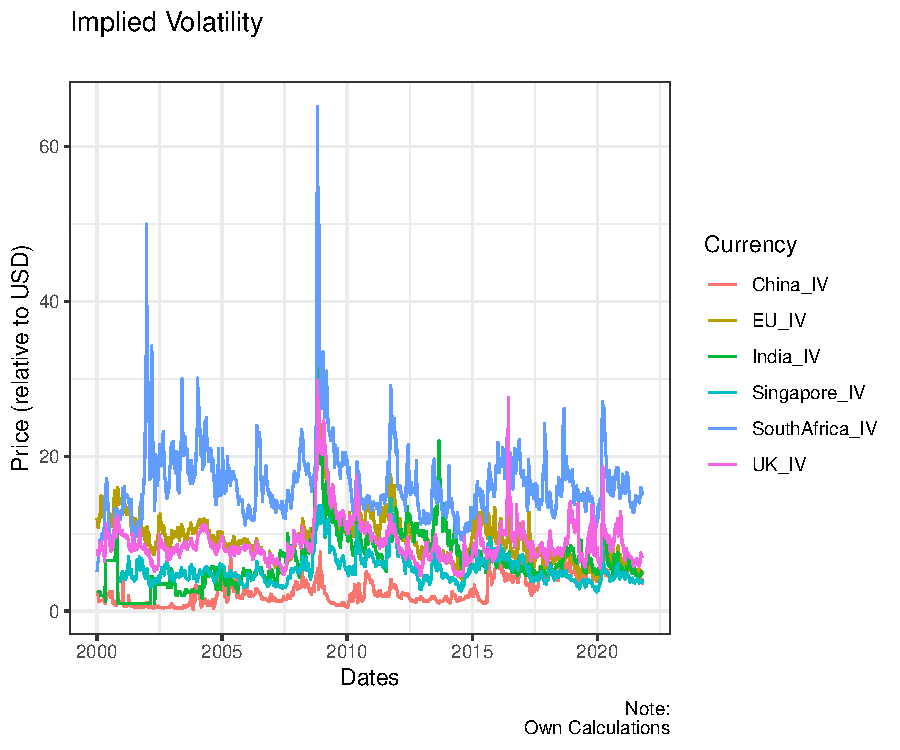
\includegraphics{Question5_files/figure-latex/unnamed-chunk-3-1.pdf}

This suggests that the market foresees the highest future volatility for
the Rand, for this sub-sample.

This suggests that the market foresees the highest future volatility for
the Rand {[}for this sub-sample{]}.

Now I'll calculate the returns to analyse the Auto-Persistence in
Returns

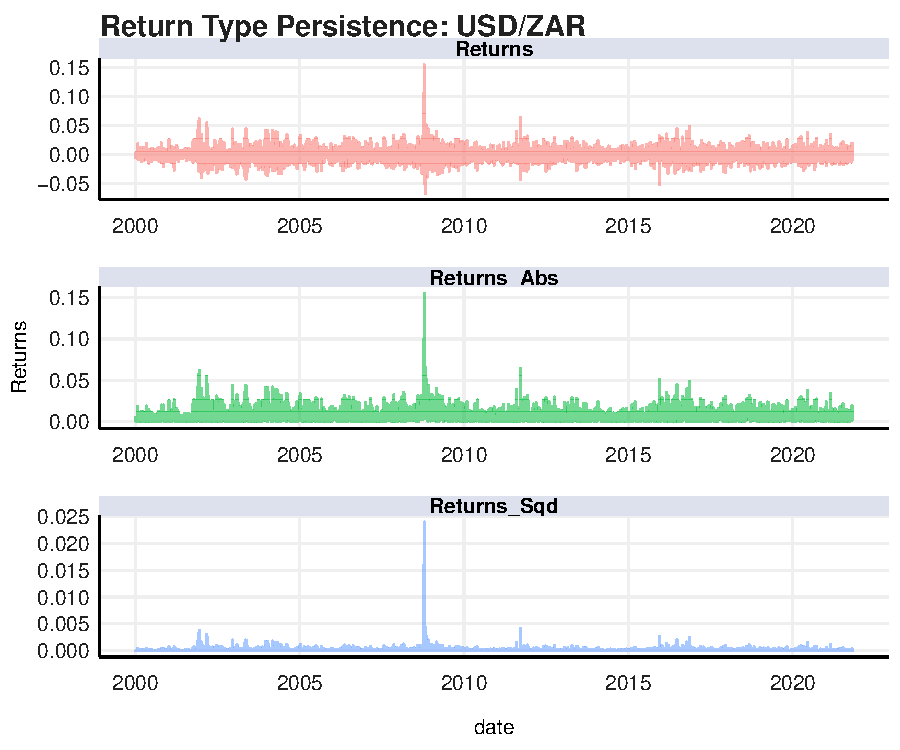
\includegraphics{Question5_files/figure-latex/unnamed-chunk-5-1.pdf}

From the graph above it is clear that there is persistence in certain
periods of USDZAR returns. Moreover, we have first and second order
persistence as well as clear evidence of long-term memory in the second
order process.

Let's investigate further\ldots{}

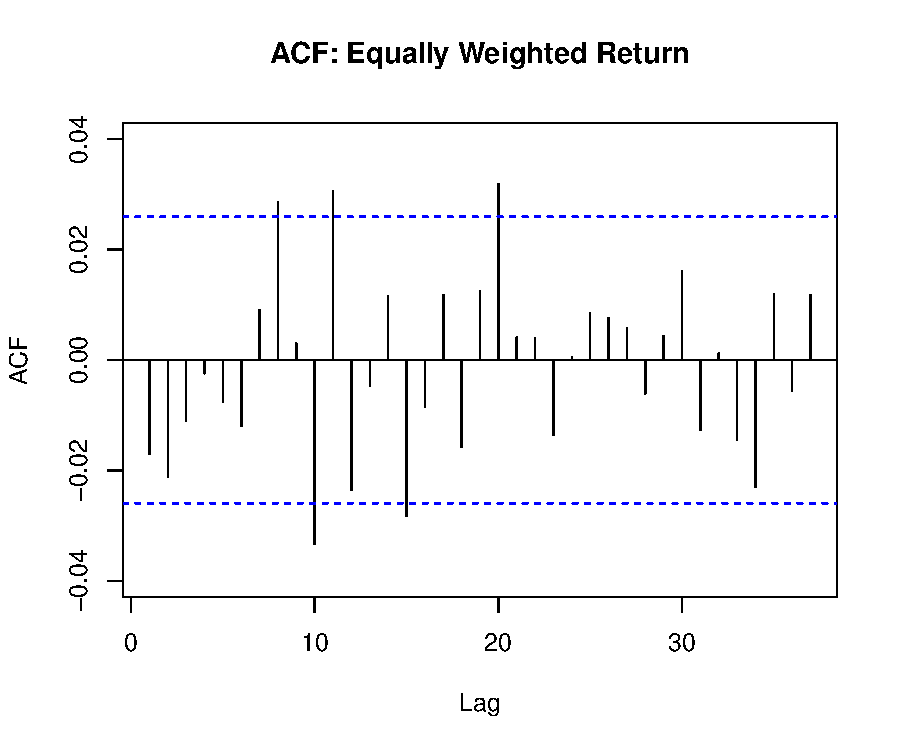
\includegraphics{Question5_files/figure-latex/unnamed-chunk-6-1.pdf}

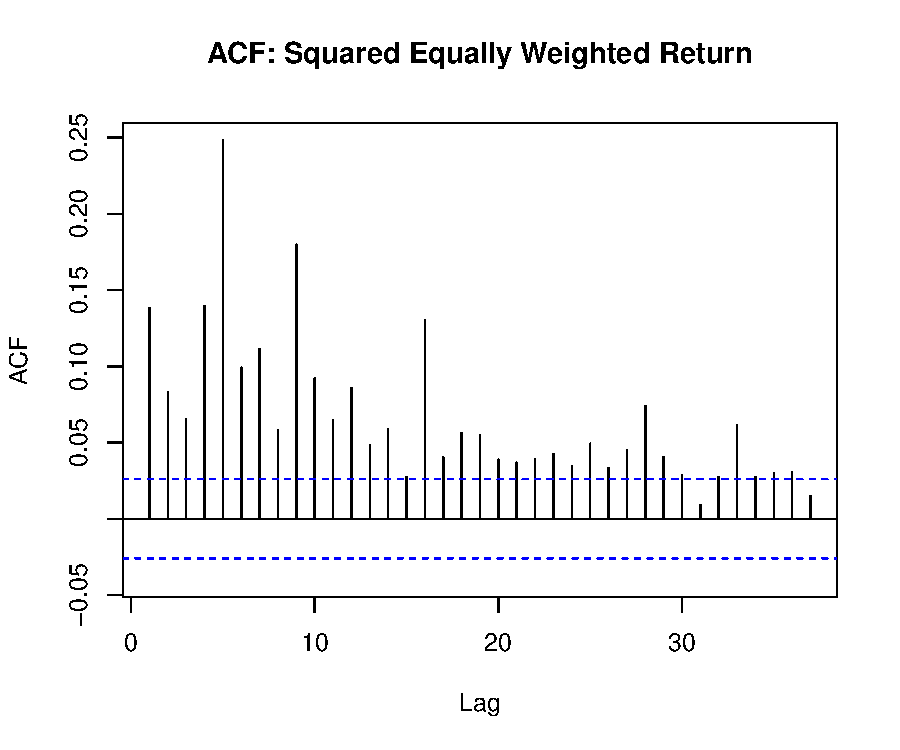
\includegraphics{Question5_files/figure-latex/unnamed-chunk-7-1.pdf}

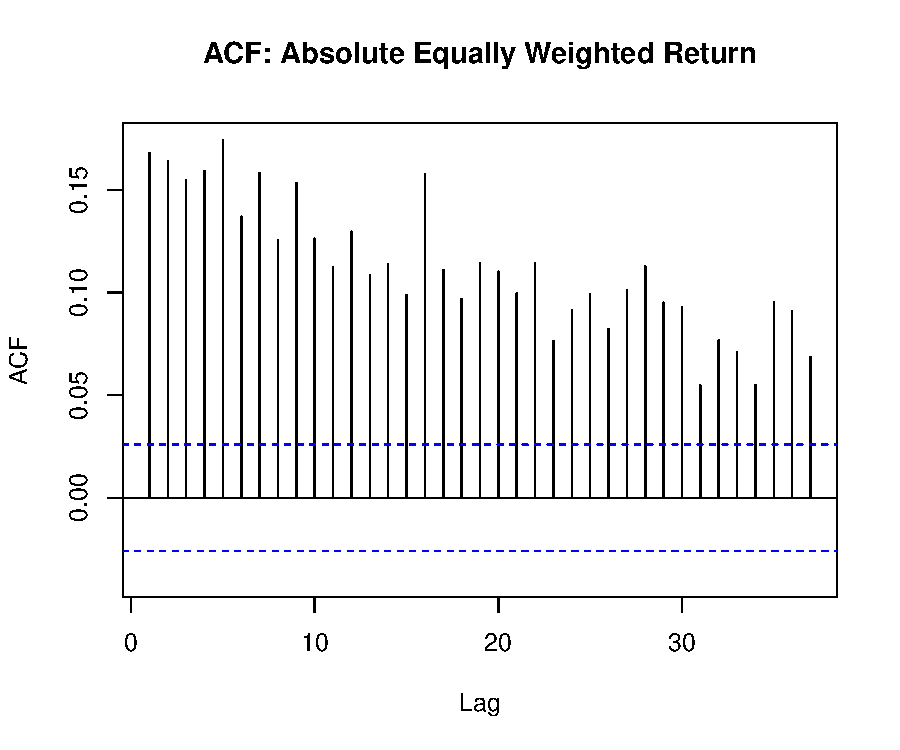
\includegraphics{Question5_files/figure-latex/unnamed-chunk-8-1.pdf}

\hypertarget{fit-model}{%
\section{Fit Model}\label{fit-model}}

\begin{table}[ht]
\centering
\begin{tabular}{rrrrr}
  \hline
 &  Estimate &  Std. Error &  t value & Pr($>$$|$t$|$) \\ 
  \hline
mu & 0.00029 & 0.00012 & 2.3906 & 0.0168 \\ 
  ar1 & -0.00039 & 0.01383 & -0.0282 & 0.9775 \\ 
  omega & 0.00000 & 0.00000 & 2.7404 & 0.0061 \\ 
  alpha1 & 0.07925 & 0.00543 & 14.5894 & 0.0000 \\ 
  beta1 & 0.92896 & 0.00748 & 124.1921 & 0.0000 \\ 
  gamma1 & -0.03796 & 0.00803 & -4.7290 & 0.0000 \\ 
   \hline
\end{tabular}
\end{table}

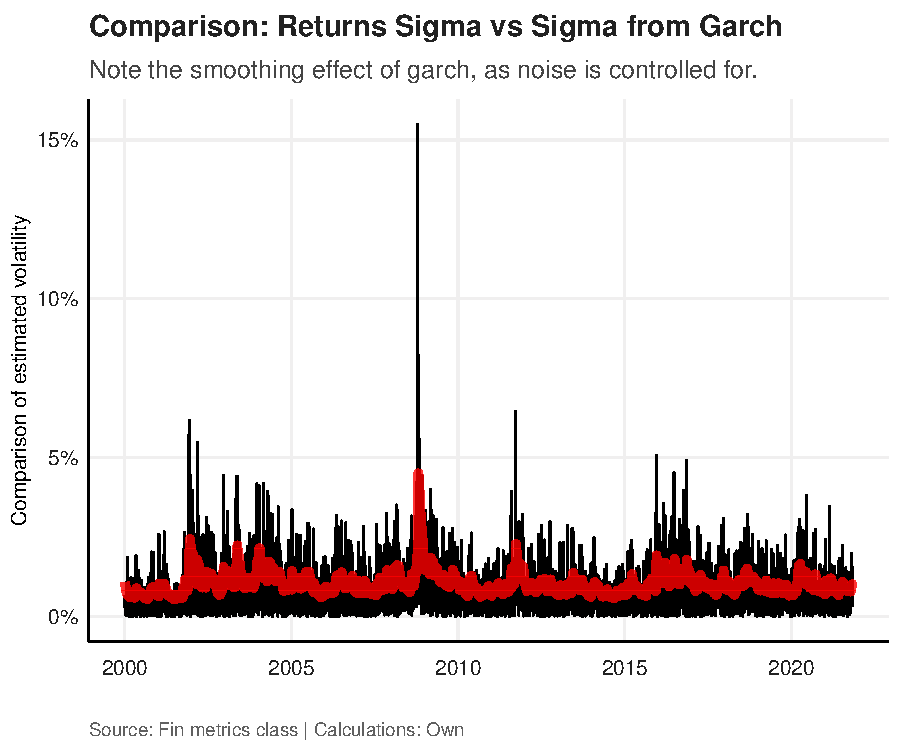
\includegraphics{Question5_files/figure-latex/unnamed-chunk-13-1.pdf}

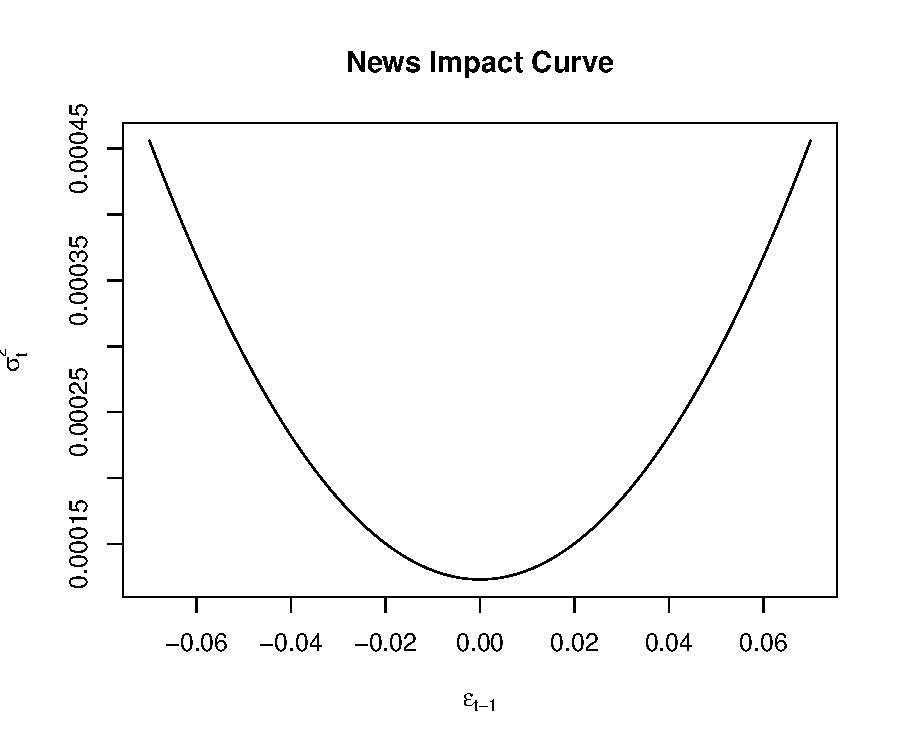
\includegraphics{Question5_files/figure-latex/unnamed-chunk-14-1.pdf}

\begin{verbatim}
## 
## please wait...calculating quantiles...
\end{verbatim}

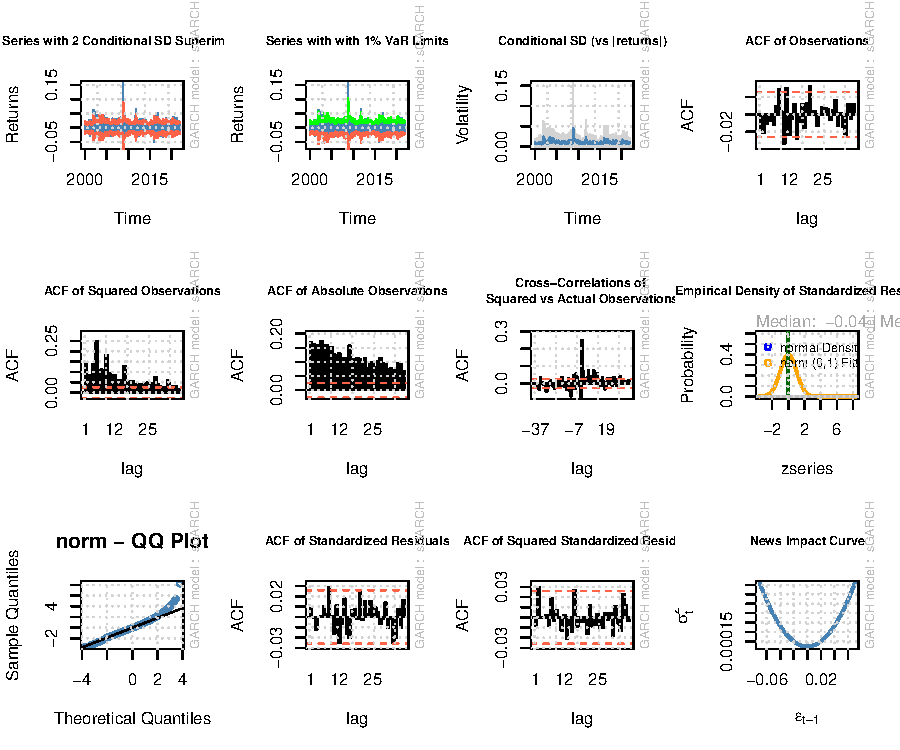
\includegraphics{Question5_files/figure-latex/unnamed-chunk-15-1.pdf}

Lets investigate further by compare smoothed ZAR Volatility to mean
Global volatility

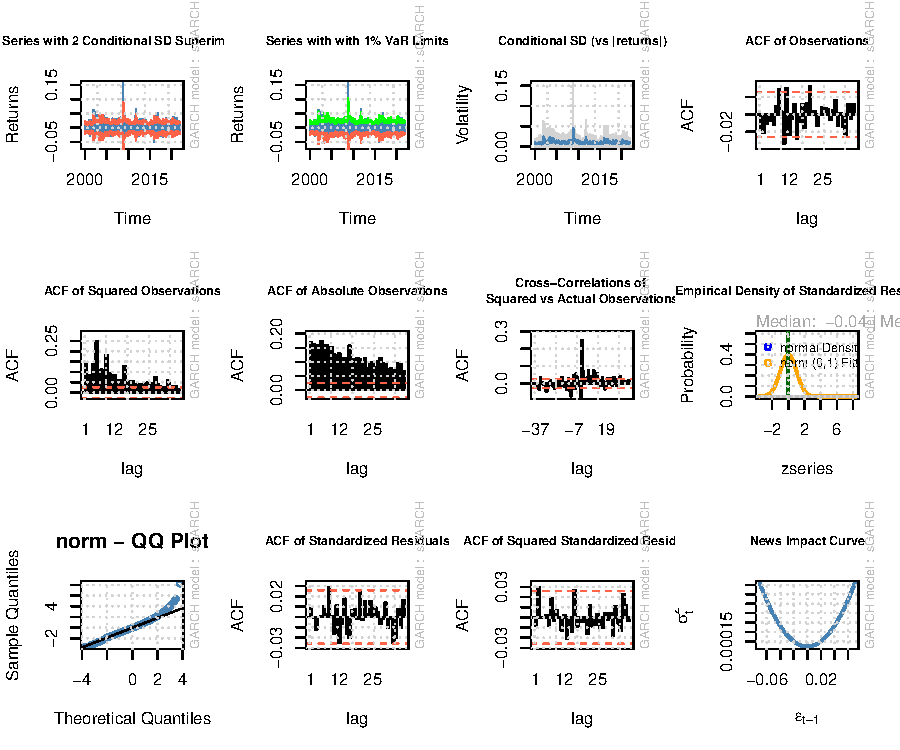
\includegraphics{Question5_files/figure-latex/unnamed-chunk-16-1.pdf}

\newpage

\hypertarget{references}{%
\section*{References}\label{references}}
\addcontentsline{toc}{section}{References}

\hypertarget{refs}{}
\begin{CSLReferences}{0}{0}
\end{CSLReferences}

\hypertarget{appendix}{%
\section*{Appendix}\label{appendix}}
\addcontentsline{toc}{section}{Appendix}

\hypertarget{appendix-a}{%
\subsection*{Appendix A}\label{appendix-a}}
\addcontentsline{toc}{subsection}{Appendix A}

Some appendix information here

\hypertarget{appendix-b}{%
\subsection*{Appendix B}\label{appendix-b}}
\addcontentsline{toc}{subsection}{Appendix B}

\bibliography{Tex/ref}





\end{document}
